\documentclass[12pt, a4paper]{article}

\makeatletter
\begingroup\endlinechar=-1\relax
       \everyeof{\noexpand}%
       \edef\x{\endgroup\def\noexpand\homepath{%
         \@@input|"kpsewhich --var-value=HOME" }}\x
\makeatother

\def\overleafhome{/tmp}% change as appropriate
\usepackage{fontspec}
\ifx\homepath\overleafhome
\setmonofont{CONSOLA.TTF}[
BoldFont=CONSOLAB.ttf,
ItalicFont=CONSOLAI.ttf,
BoldItalicFont=CONSOLAZ.ttf
]
\else
\setmonofont{Consolas}
\fi

\usepackage[onehalfspacing]{setspace}
\parskip=1mm plus 1pt
\usepackage{indentfirst}
\usepackage{forest}
\usepackage[export]{adjustbox}
\usetikzlibrary{arrows.meta, %提供Stealth[]箭头类型
angles} %提供angle pic
	\forestset{
	tree angle/.style={
		% !表示开始相对引用。u是父节点,n是下一个兄弟节点。他们都是short-form step。
		% pic {angle}: draw a small picture of type angle.
		% angle是来自\usetikzlibrary{angles}。
		% The angle pic draws an angle between the two lines BA and BC, where A, B, and C are three coordinates.
		tikz={\path () coordinate (A) -- (!u) 
			coordinate (B) -- (!n) 
			coordinate (C) pic [draw, angle radius=#1] {angle};}
	},
	tree angle/.default=5mm
}

\usepackage[section]{placeins}

\usepackage{xcolor}
\usepackage{algorithm}
\usepackage{algorithmic}
\usepackage{makeidx}
\usepackage{hyperref}
\hypersetup{
unicode=true,          % non-Latin characters in Acrobat’s bookmarks
pdftitle={},    % title   
%pdfauthor={爱让一切都对了},     % author   
%pdfcreator={爱让一切都对了},
%pdfproducer={OpenOffice.org 3.3},
breaklinks=true,
colorlinks=true,       % false: boxed links; ture: colored links
linkcolor=blue,          % color of internal links   
citecolor=blue,        % color of links to bibliography  
filecolor=magenta,      % color of file links   
urlcolor=cyan,           % color of external links  
}
\usepackage{xcolor}

\usepackage{url}
\def\UrlBreaks{\do\A\do\B\do\C\do\D\do\E\do\F\do\G\do\H\do\I\do\J\do\K\do\L\do\M\do\N\do\O\do\P\do\Q\do\R\do\S\do\T\do\U\do\V\do\W\do\X\do\Y\do\Z\do\[\do\\\do\]\do\^\do\_\do\`\do\a\do\b\do\c\do\d\do\e\do\f\do\g\do\h\do\i\do\j\do\k\do\l\do\m\do\n\do\o\do\p\do\q\do\r\do\s\do\t\do\u\do\v\do\w\do\x\do\y\do\z\do\0\do\1\do\2\do\3\do\4\do\5\do\6\do\7\do\8\do\9\do\.\do\@\do\\\do\/\do\!\do\_\do\|\do\;\do\>\do\]\do\)\do\,\do\?\do\'\do+\do\=\do\#}

\usepackage{listings}
\lstset{
%  %行号
%  %numbers=left,
%  %背景框
%  %framexleftmargin=10mm,
%  %frame=none,
%  %背景色
%  %backgroundcolor=\color[rgb]{1,1,0.76},
%  %样式
  keywordstyle=\color{blue}\bfseries,
%  identifierstyle=\bf,
%  numberstyle=\color[RGB]{0,192,192}, %行号的样式
  commentstyle=\it\color[RGB]{0,96,96},
  stringstyle=\rmfamily\slshape\color[RGB]{128,0,0},
%  %显示空格
%  %showstringspaces=false,
  basicstyle=\ttfamily\footnotesize, %修正大写字母间距过小
  columns=flexible, %修正大写字母间距过小
  breaklines=true, %对过长的代码自动换行
%  escapechar=!,
%  morekeywords={BEGIN}
    upquote=true,
  language=python
}

\newcommand{\code}[1]{\texttt{#1}}
\newcommand{\citeWeb}[3]{#1, \url{#2}, Retrieved #3.}
\title{CS 188 Security Evaluation on Team Random's Project}
\author{Weikeng Yang\\405346443 \and
Yingzhe Hu\\505366341 \and
Qiqi Gu\\604253019 \and
Dongyao Liang\\705313832 \and
Shuhua Zhan\\705190671}
\date{Team name: Random\\[2mm]February 28, 2020}

\usepackage[numbers]{natbib}
\setcitestyle{square}

\usepackage{graphicx}
\makeindex

\begin{document}

\maketitle
\printindex

\section{Summary}

\index{Summary}
This report evaluates our own project, Google Play Advanced Search.

Requirement: A brief summary of your findings, including the approach(es) you took and what you learned. This should be at a high level (e.g., "Working from the design document, we decided to perform code review using the following techniques, supplemented by the following kinds of testing") and should include some conclusion about the security of the system (e.g., "Our analysis showed that the mitigations used to address security concerns in our system were effective," or "Our analysis reveals fatal security flaws that could be remediated in the following ways," or a statement of similar nature).   For evaluation of the other team’s project, remember that your goal is not to criticize their efforts, but to determine whether they achieved sufficiently secure results and to suggest improvements if they did not. 

\section{Security Evaluation Plan}

\index{Security Evaluation Plan}
Requirement: A description of your plan for the security evaluation, including steps to be taken, tools or approaches used, work assignments, and a schedule. Since it is likely that your plan required some adjustments, you should discuss the degree to which you followed your plan versus deviating from it, as well as explanations for such deviations.  

We plan to evaluate two parts of project Google Play Advanced Search, namely the source code, and the application deployed to Google Cloud, accessible via \url{https://beta.gqqnbig.me/}. We will check the security issues in the source code, and find if the server is properly protected.

When we were developing the project, we were already performing code review, ie. a team member creates pull requests (PR) for his/her changes, and an experienced team member will review the commits in the pull requests, approve the PR or request revisions. However, it is mainly Qiqi and Dongyao who review pull requests. We will ask other team members to read the code in hope that they find out something the PR reviewer missed before.

When we are doing security evaluation code review, candidate point strategies.

We will also check the security vulnerabilities of the dependencies of the project.

Our plan for the security evaluation as follow:
\begin{itemize}
    \item Security Design Review
    \item Code Review and External Packages
    \item Testing
    
Testing is one important element of our evaluation. We plan to use these testing tools:
\begin{itemize}
    \item Network sniffers
    \item \code{Nmap} as Port scanners
    \item \code{OWASP ZAP} for Web security testing 
%    \item Tools to test crypto usage
    \item Fuzz testing tools
%    \item Password crackers
%    \item Database security scanners
%    \item Mobile app security testers (MASTs)
    \item Interactive application security testing (IAST)
\end{itemize}
\end{itemize}



\section{Security Evaluation Results}

\index{Security Evaluation Results} 
Requirement: You should describe the results of your security evaluation, providing sufficient details to justify any conclusions you reach. This section should be significantly more extensive than the summary, containing a great deal more detail. If, for example, you found a dangerous race condition in the code, you should describe how you found it, what the security implications are, and suggest approaches for fixing it or ensuring that it is not exploited. 

\subsection{Security Design Review}
\begin{figure}[ht]
\centering
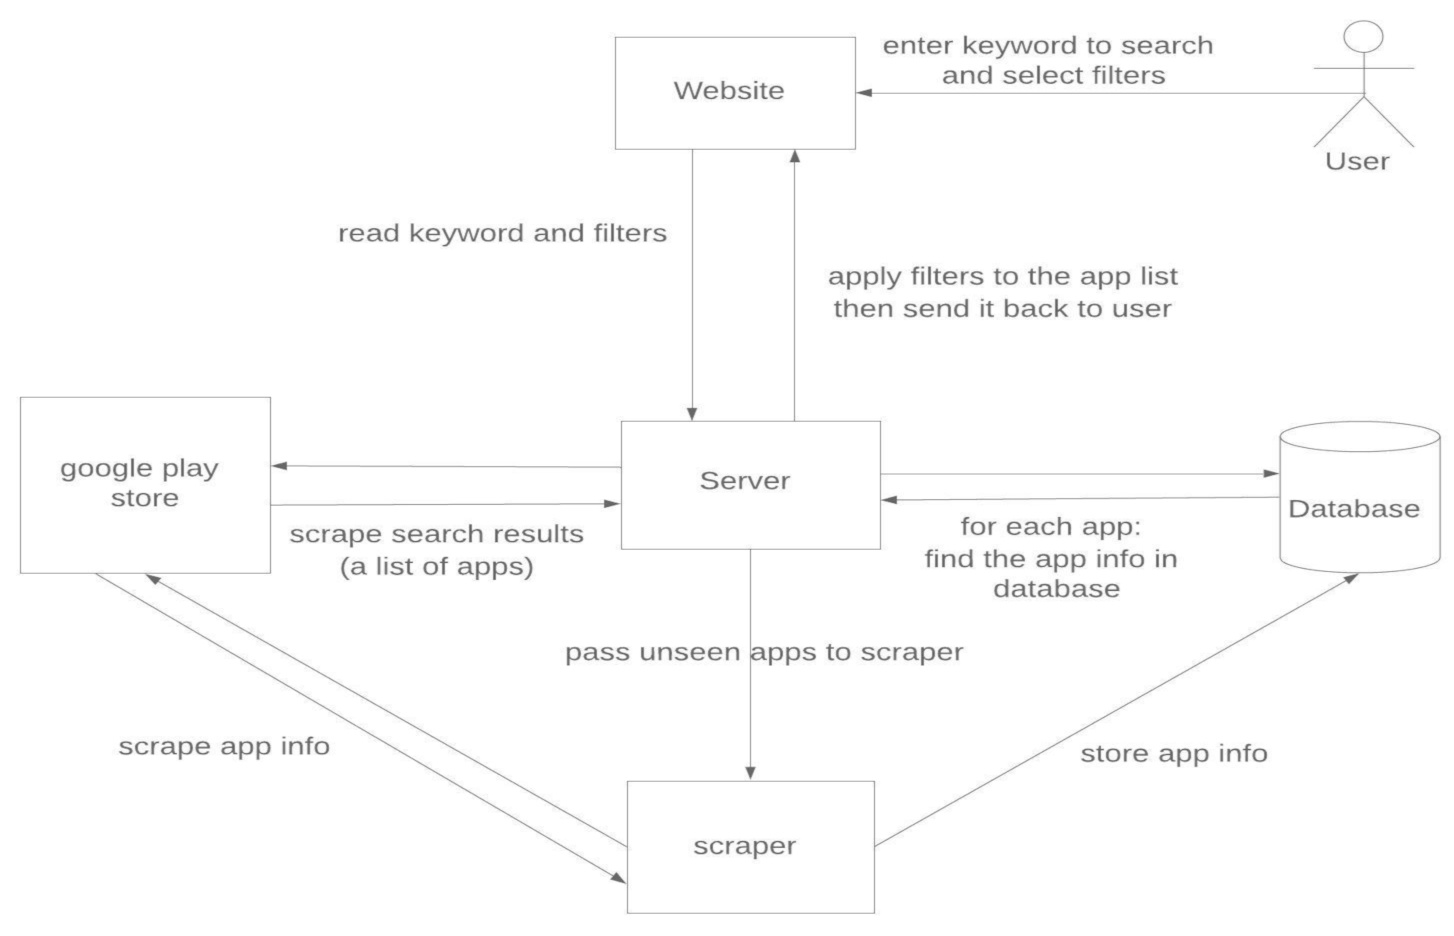
\includegraphics[width=\textwidth]{Context_Diagram.jpeg}
\caption{Design Diagram}
\label{fig:design_diagram}
\end{figure}

Figure \ref{fig:design_diagram} is the design diagram. We evaluate the design again. By looking at the source code at a high level, we conclude the implemented project largely matches the design, with a few exceptions.

\begin{figure}[ht]
\centering
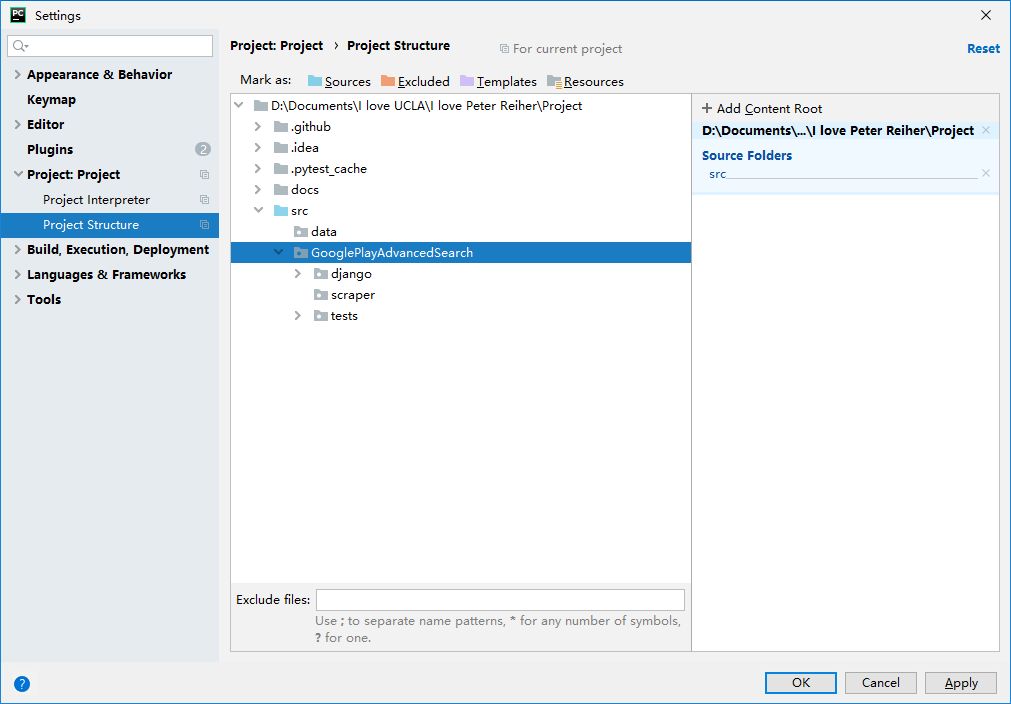
\includegraphics[width=\textwidth]{project-structure.png}
\caption{Project structure. \code{src} is the source code root.}
\label{fig:project-structure}
\end{figure}

The implemented project has 3 modules, well organized into a hierarchical namespace, see Figure \ref{fig:project-structure}. \code{src} is the source code root. tests is the additional module but since it's for automated tests, the addition is not a big deal.

The design diagram indicates there is a server component, but actually the django module and the scraper module both run on a server; the SQLite database is on the same server as well. Some functions, for instance \code{src/GooglePlayAdvancedSearch/DBUtils.py} are shared across modules. 

Unlike the design diagram, the implemented website talks to database, and run scraper as a standalone process. Both are found in \linebreak[4]
\code{GooglePlayAdvancedSearch\linebreak[0].django.web.Api}\footnote{All code are in namespace \code{GooglePlayAdvancedSearch}. Moveing forward, we will remove this prefix for conciseness and only say \code{django.web.Api}.}.

Moreover, the django module has some scraping abilities. It scrapes Google Play search result page, and if the module requires more information, it then calls scraper.

By looking at the design, we hold the threats to the application are: 1) Attackers attacking through the website; 2) Attackers attacking the server; 3) Malicious data injected from Google Play. There are also threats to end users: 4) Attackers may perform man-in-the-middle attack. 5) We have to prevent cross-site attack, and 6) check client side security vulnerabilities, mainly JavaScript.

We assign high priority to 1), 5); medium to 4), 6), low to 2), 3).

% data flow 
\begin{figure}[ht]
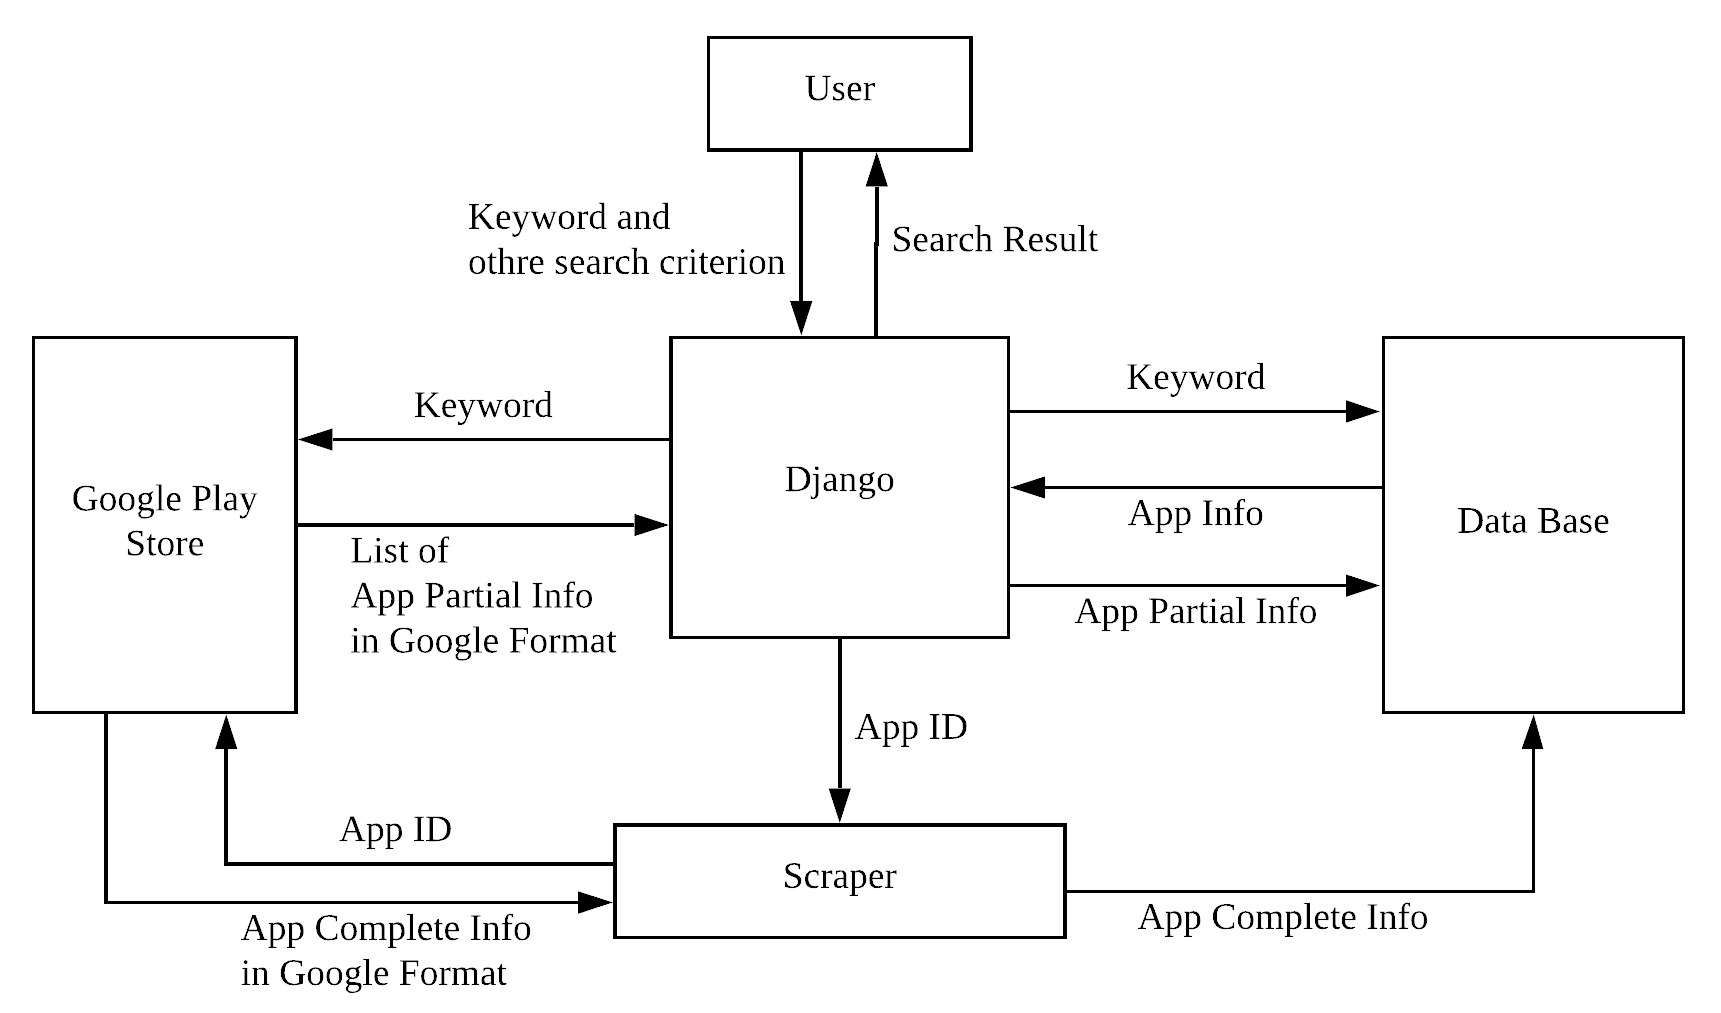
\includegraphics[width=\textwidth]{dataFlow.png}
\caption{Data Flow Diagram}
\label{fig:dataFlow}
\end{figure}

Additional, we also check and review the process of data flow. When an user uses our website(Google Play Advanced Search) to search some specific Apps, the data flow will show as the diagram. 1) Django sends the request to Google Play Store based on the user's search keywords and gets the partial information of apps back(Apps ID). 2) Django sends all the apps ID and the filtering information for user to database and try to get corresponding complete information of apps. 3) If Django makes sure that our database have all the information of apps which are searched from Google Play Store, it just return the results to the user directly. 4) Otherwise, Django will record the missing apps ID and pass them to Scraper. 5) Scraper goes to Google Play Store to get complete information of the missing apps and save all the new data in database. 6) Finally, Django grabs all the complete information from database and returns them to user.

Based on the process of data flow, we found that the most likely security issues - trace malicious input. We try to do some fuzz testings. 

\code{requirements.txt} lists the Python packages not developed by us. In addition, we use SQLite database and some client-side JavaScript libraries. Section \ref{dependency-evaluation} evaluates the security of these dependencies.

\subsection{Code Review}
code review approach
top down? bottom up?
While reviewing our codes, we performed top-down approach where we start with the general framework of the codes and then look deeper into specific functions.

We used Candidate point strategies, searching for \code{StringAgg(delimiter)}, which is subject to SQL injection.



% https://developer.mozilla.org/en-US/docs/Learn/Server-side/Django/web_application_security

We are running Django as our framework, so it is good to know about the protection and potential threats provided by Django.
\begin{itemize}
    \item Cross site scripting(XSS). Django's template system protects us against the majority of XSS attacks by escaping specific characters that looks dangerous in HTML. For example the string "<script>" will be turned into "\textcolor{blue}{\&lt}script\textcolor{blue}{\&lt}".
    \item Django provides some CSRF protection by invoking \code{\{\% csrf\_token \%\}} tag into form definition although we don't have any form requests.
    \item SQL injection protection. Django’s querysets are protected from SQL injection since their queries are constructed using query parameterization. A query’s SQL code is defined separately from the query’s parameters. In additional, we have written some raw queries and we need to make sure they are secure from SQL injection (we will talk about it below)
    \item Django can be configured to enforce SSL. With enabling SSL, we can use \code{SECURE\_PROXY\_SSL\_HEADER} to check if the incoming content is secure; \code{SECURE\_SSL\_REDIRECT} to redirect all http to https, (we configure a non-https to https redirection on nginx in our production server instead); and \code{SESSION\_COOKIE\_SECURE} to make sure cookies are only sent over http and \code{SESSION\_COOKIE\_SECURE} to make sure cookies are only sent over https.
\end{itemize}


We looked at the SQL injection possibility on the search box. The handler of the request is at \code{django.web.Api.search()}. We notice the user input keyword is passed into two places, namely \code{DBUtils.AppAccessor.\linebreak[0]searchApps()} and \code{django.web.Api.searchGooglePlay()}. Listing \ref{lst:searchApps} is an extract of \code{django.web.Api.searchGooglePlay()}, where a severe denial of service issue exists.

\begin{lstlisting}[frame=tb, caption=DBUtils.AppAccessor.searchApps(), label=lst:searchApps]
def searchApps(self, namePattern: str) -> List[AppItem]:
	appList = []

	self.__cursor.execute("SELECT id,name,rating,num_reviews,install_fee,inAppPurchases,app_icon FROM App WHERE name LIKE :namePattern", {"namePattern": '%' + namePattern + '%'})
\end{lstlisting}

Neither the searchApps function or the call sites verifies the length of parameter namePattern. Initially on the website, user has to type something to make the search button enabled, which might be the safe guard against searching for an empty keyword, see Figure \ref{fig:website-gray-buton}. However, if the user deletes the keyword, the search button is still enabled. Therefore user is able to search for an empty keyword, and the SQL statement doesn't limit the return rows. If there are many data in database, all data will be returned, and the execution time might be long. It can potentially become a denial of service.


\begin{figure}[ht]
\centering
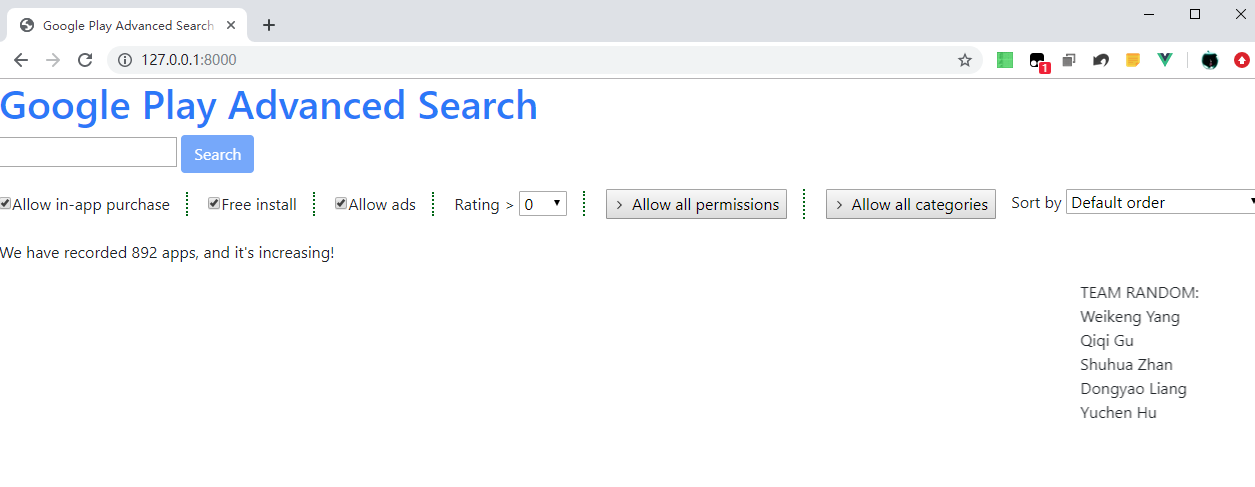
\includegraphics[width=\textwidth]{website-gray-button.png}
\caption{Initially the website has a disabled search button, but user can type something then delete them, enabling searching for empty keyword.}
\label{fig:website-gray-buton}
\end{figure}

\subsection{Automated Tests}
Project Google Play Advanced Search comes with a number of automated tests located in the tests module. These are all functional tests and the badge on the README file on the repository confirms the code passes all tests. However, there are no security tests there.



\subsection{Tool Testing Results}
\subsubsection{Nmap for Port Scanning}
We use Nmap to scan the open ports on our server. Currently we have a public ip \textcolor{green}{35.236.119.106} and domain beta.gqqnbig.me

Running Nmap with \code{-p-} flag to scan all 65535 ports on our server.
We find these ports are open:
\begin{center}
    \begin{tabular}{l l l}
        PORT & STATE & SERVICE \\
        22/tcp & open & ssh\\
        80/tcp & open & http\\
        443/tcp & open & https
    \end{tabular}
\end{center}

These are exactly all ports we need to use. We didn't leave any unused port open. Detail output see fig \ref{fig:nmap}.

\begin{figure}[H]
\centering
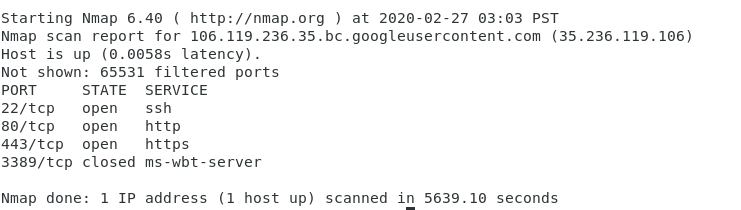
\includegraphics[width=\textwidth, frame]{nmap_log.png}
\caption{Nmap Output}
\label{fig:nmap}
\end{figure}

\subsubsection{OWASP ZAP}
ZAP is a open source project developed by OWASP. It can help us to find the some potential security problems of our web server like SQL injection, XSS and many others.
We run zap to attack our website home page and found some Alerts:
\begin{itemize}
    \item Risk: \textcolor{orange}{low}. Cross-Domain JavaScript Source File Inclusion. We are using some third-party javascript libraries. They are:
    \begin{itemize}
        \item jQuery API:\\ \textcolor{blue}{<script src="https://code.jquery.com/jquery-3.4.1.min.js"></script>}
        \item A CDN for npm - lodash:\\ \textcolor{blue}{<script src="https://cdn.jsdelivr.net/npm/lodash@4.17.15/lodash.min.js"></script>}
        \item A progressive javascript framework - Vue.js:\\ \textcolor{blue}{<script src="https://cdn.jsdelivr.net/npm/vue@2.6.11"></script>}
    \end{itemize}
%    \item Risk: \textcolor{orange}{low}. Incomplete or No Cache-control and Pragma HTTP Header Set
%    \item Risk: \textcolor{orange}{low}. X-Content-Type-Options Header Missing on file \code{static/js/vue-click-outside.js} and \code{static/images/question.png}
    \item Risk: \textcolor{blue}{Informational}. Information Disclosure - Suspicious Comments
    \item Risk: \textcolor{blue}{Informational}. Timestamp Disclosure - Unix
\end{itemize}
One way to work around the first alert is by deploying the production mode of above third party javascript libraries to reduce the potential threat if we have more time.

Then we use ZAP to attack our search pages \\(eg. https://beta.gqqnbig.me/search?q=youtube&pids=33&cids=55,57) with some permission and category filters.
And we discover more alerts (fig \ref{fig:zap-alerts}).

\begin{figure}[H]
\centering
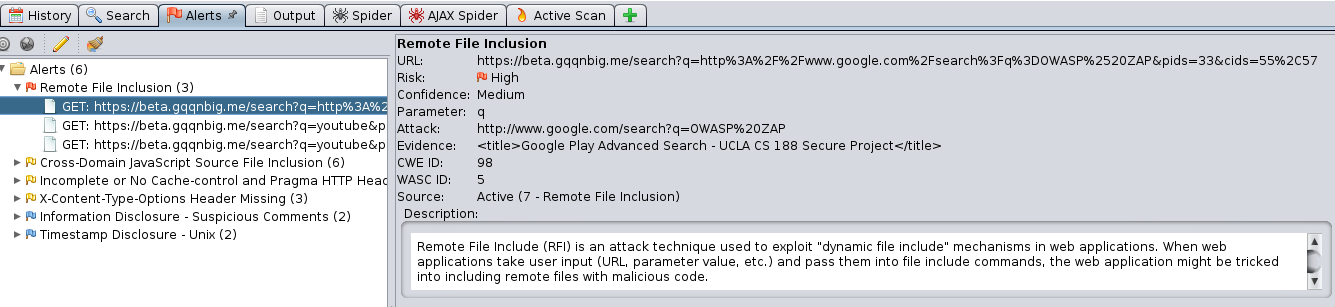
\includegraphics[width=\textwidth, frame]{zap_alerts.png}
\caption{ZAP Alerts}
\label{fig:zap-alerts}
\end{figure}

In this case, it has a \textcolor{red}{High} risk alert: \code{Remote File Inclusion}










\section{Recommendations for future evaluations}

\index{Future evaluations} 
Requirement: If time and resources did not permit you to study the system as fully as you feel was desirable, you should discuss how future efforts to better understand the security of the system should be directed. You should also discuss conditions under which a fresh review might be required, such as the addition of obvious major extensions to the prototype of the project. 

\section{Lessons learned by performing the security evaluation}

\index{Lessons learned}
Requirement: Beyond learning something about the security of the project, we hope you will learn something about designing secure systems, secure coding, and evaluating the security of systems. In this section, discuss what you have learned.  

\section{Work breakdown}

\index{Work breakdown}
Requirement:  Indicate exactly which elements of the report and work required to produce it were performed by each team member. 

Shuhua Zhan - responsible for lessons learned section of the report and participated in code review. In the project, participated in element \code{app\_icon}, fixed problem when no results find in google play website and improved the user interface of the website.

\section{Supplementary materials}

\index{Supplementary materials}
Requirement: If your analysis produced useful artifacts (such as automated reports, screen shots demonstrating problems, scripts used to test functionality, etc.), include these in appendices, where possible. For things that are not easily embedded in a 
report (such as a video demonstrating how to exploit a security flaw), upload them as separate files when you submit the report. You can also provide links to supplementary materials, but if you do, make sure that the materials are in a location that can be accessed by others, not in a private area. Make sure that your supplementary material section indicates which files are uploaded as part of your report, which links are associated with your report, and what each file or link represents.  
 

\end{document}